% Created 2026-08-31 Mon 01:17
% Intended LaTeX compiler: xelatex
\documentclass{article}

\usepackage{amsmath}
\usepackage{fontspec}
\usepackage{graphicx}
\usepackage{longtable}
\usepackage{wrapfig}
\usepackage{rotating}
\usepackage[normalem]{ulem}
\usepackage{capt-of}
\usepackage{hyperref}
\newcommand{\avg}[1]{\langle #1 \rangle}
\usepackage{amsmath}
\usepackage{amssymb}
\usepackage[thinc]{physics}
\usepackage{geometry}
\geometry{left=2.5cm,right=2.5cm,top=2.5cm,bottom=2.5cm}
\usepackage{xcolor}
\usepackage[unicode]{hyperref}
\hypersetup{
colorlinks=true,
linkcolor=blue,
citecolor=blue,
urlcolor=blue
}
\urlstyle{same} % keep URL font same as main text
\author{Soroush Seirani G.}
\date{\today}
\title{Avalanche's Progress Report 4}
\hypersetup{
 pdfauthor={Soroush Seirani G.},
 pdftitle={Avalanche's Progress Report 4},
 pdfkeywords={},
 pdfsubject={},
 pdfcreator={},
 pdflang={English}}
\begin{document}

\maketitle
\section{Types of Networks}
\label{sec:orgb1c7005}
\subsection{Erdos-Reyni Networks}
\label{sec:org609a910}
There are two variants of this network but I only use one of
them. This network is defined by the possiblity of each edge to
exist. We assume a constant probability \(p\) for each edge to exist and
roll our dice to construct the network.

Since the probability of each edge's existance is constant, the
expected degree is:

\begin{gather}
  \avg{k} = p(N-1) \approx pN \quad \text{for large $N$}
\end{gather}

And the probability distribution of degrees follows a binomial
distribution:

\begin{gather}
  P(k) = \begin{pmatrix}
    N-1\\
    k
  \end{pmatrix} p^k (1-p)^{N-1-k}
\end{gather}

Which due to its dependence on the system's size \(N\) isn't scale-free.
\subsection{Barbasi-Albert Networks}
\label{sec:org231968b}
This network is defined using the algorithm used to generate it:

\begin{enumerate}
\item The network is initialized with \(m \ge 2\) nodes which is usually
fully connected
\item One node is added and each edge which could be
connected to it exists with prbability:
\begin{gather}
  p_i = \frac{k_i}{\sum_j k_j}
\end{gather}
\item If the size of the system isn't yet equal to \(N\) go back to step 2.
\end{enumerate}

This gives us a scale-free network but not the most generic one. It
assumes certain properties about the network. I plan to use another
algorithm in the future to get more general results.
\section{Determining Distributions From Samples}
\label{sec:orgb89f7cd}
Currently I've implemented functions for directly picking a sample
avalanche size. By picking a big number of samples and drawing the
histogram I can observe what the probability distribution looks like
but how could I rigorously determine the probability distribution?

To address this problem I did some research and came across the
``likelihood function''. Here I'll explain what methods I used to
find the analytical expression for the measured samples.

Assume a series of experiments (direct samples) denoted by \(X_i\). The
likelihood function is defined:
\begin{gather}
  L(\boldsymbol{X}) = \prod_{i}P(X_i)
\end{gather}

Which is maximized if the function \(P\) is the right probability
distribution for our samples. So we can have a generic distribution
which depends on multiple variables \(\boldsymbol{\theta}\):
\begin{gather}
  L(\boldsymbol{X},\boldsymbol{\theta}) =  \prod_{i}P(X_i,\boldsymbol{\theta})
\end{gather}

And I can using optimization techniques to find the right
\(\boldsymbol{\theta}\) which uniquely determines the correct
distribution. Note that despite being able to compare multiple
probability distributions, we still have to provide
\(P(x,\boldsymbol{\theta})\) but that won't be a problem for us because
we can make good guesses :P

Note that if we work with \(L\) directly we'll have numerical problems
because the product of probabilities will be much smaller than the
available precision so we'll work with its logarithm:
\begin{align}
  L(\boldsymbol{X},\boldsymbol{\theta}) &=  \prod_{i}P(X_i,\boldsymbol{\theta}),\\
  \ln L(\boldsymbol{X},\boldsymbol{\theta}) &= \ln  \prod_{i}P(X_i,\boldsymbol{\theta})\\
    &= \sum_i \ln P(X_i,\boldsymbol{\theta})
\end{align}
\section{Results and Future Work}
\label{sec:orgd8ca598}
So far I've run three simulations. The resulting graphs and their descriptions are below:
\begin{center}
\begin{center}
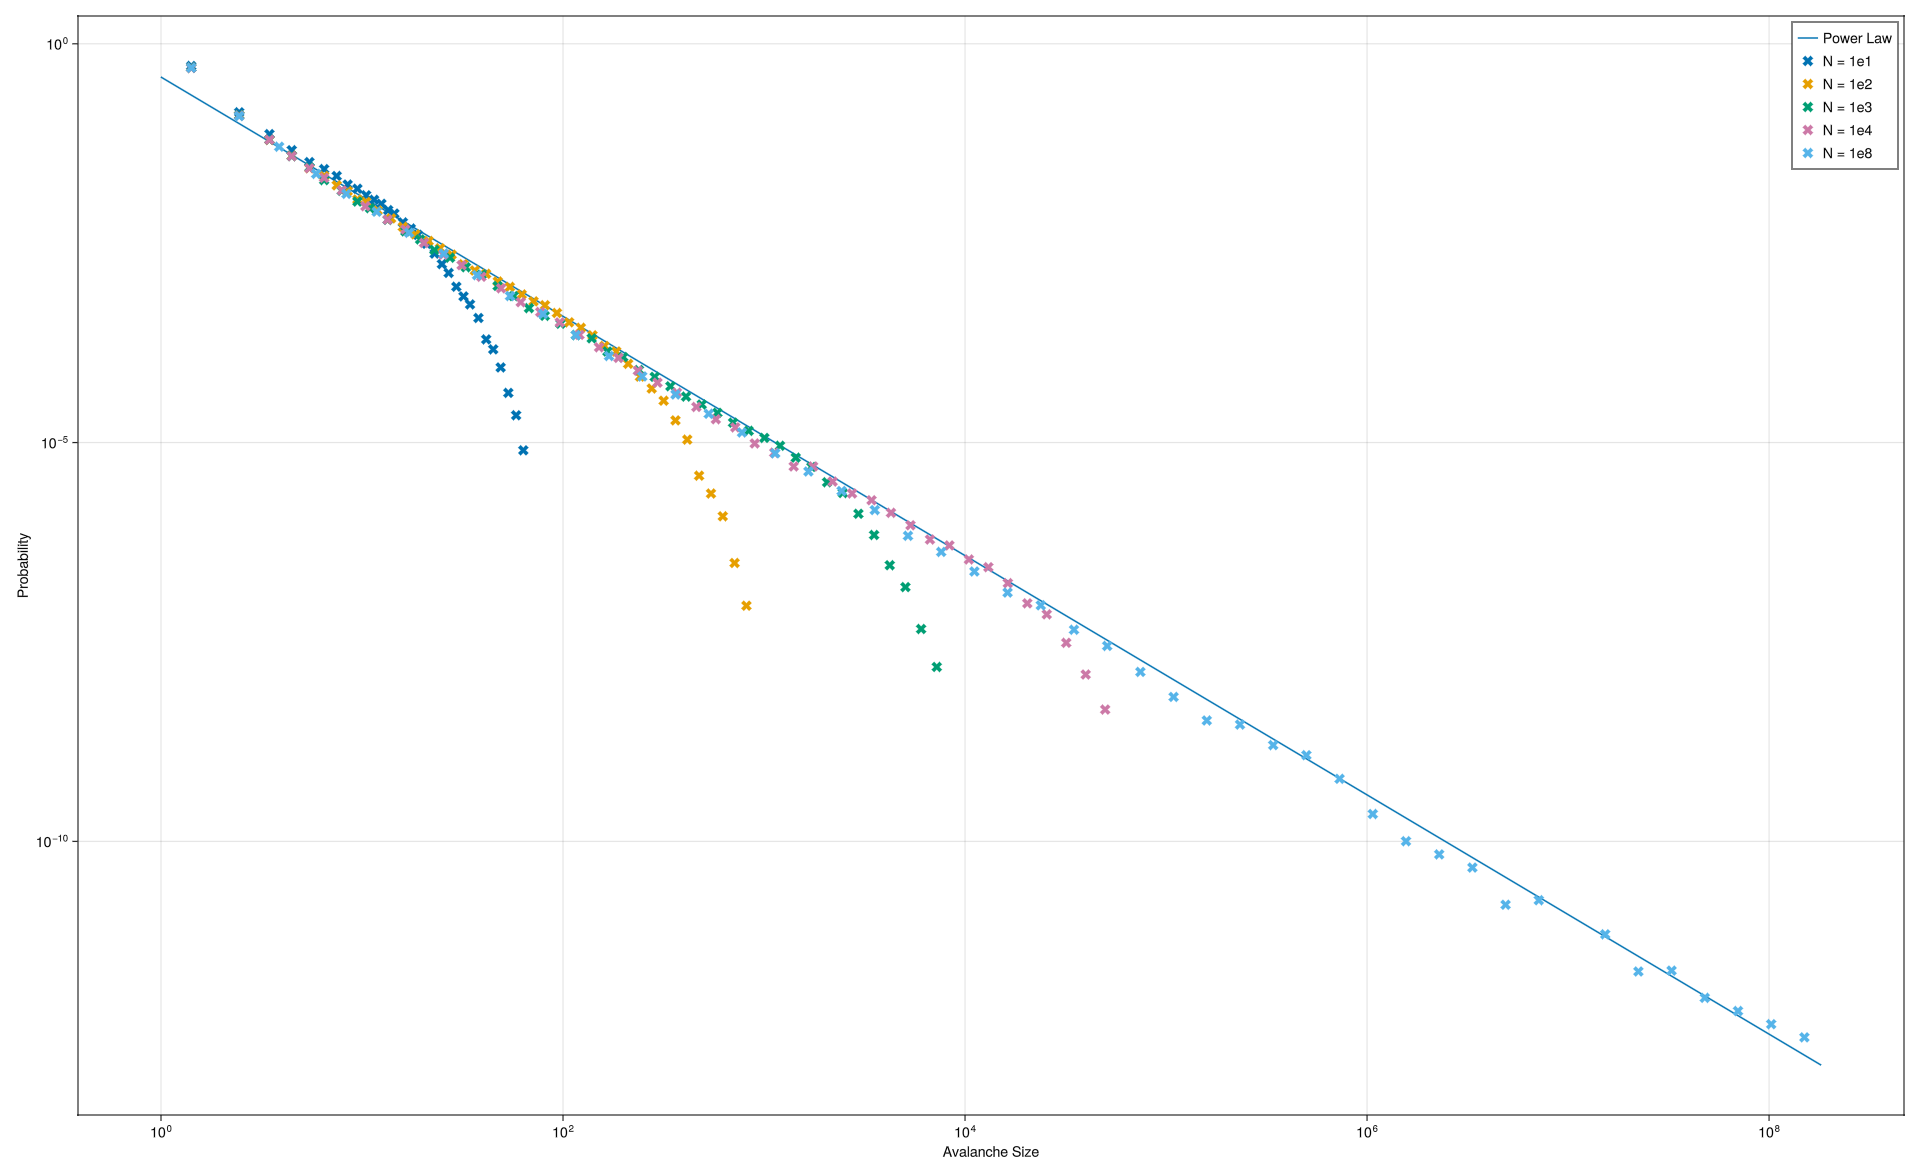
\includegraphics[width=.9\linewidth]{fig1.png}
\end{center}
Fully Connected Network with Variable System Size
\begin{center}
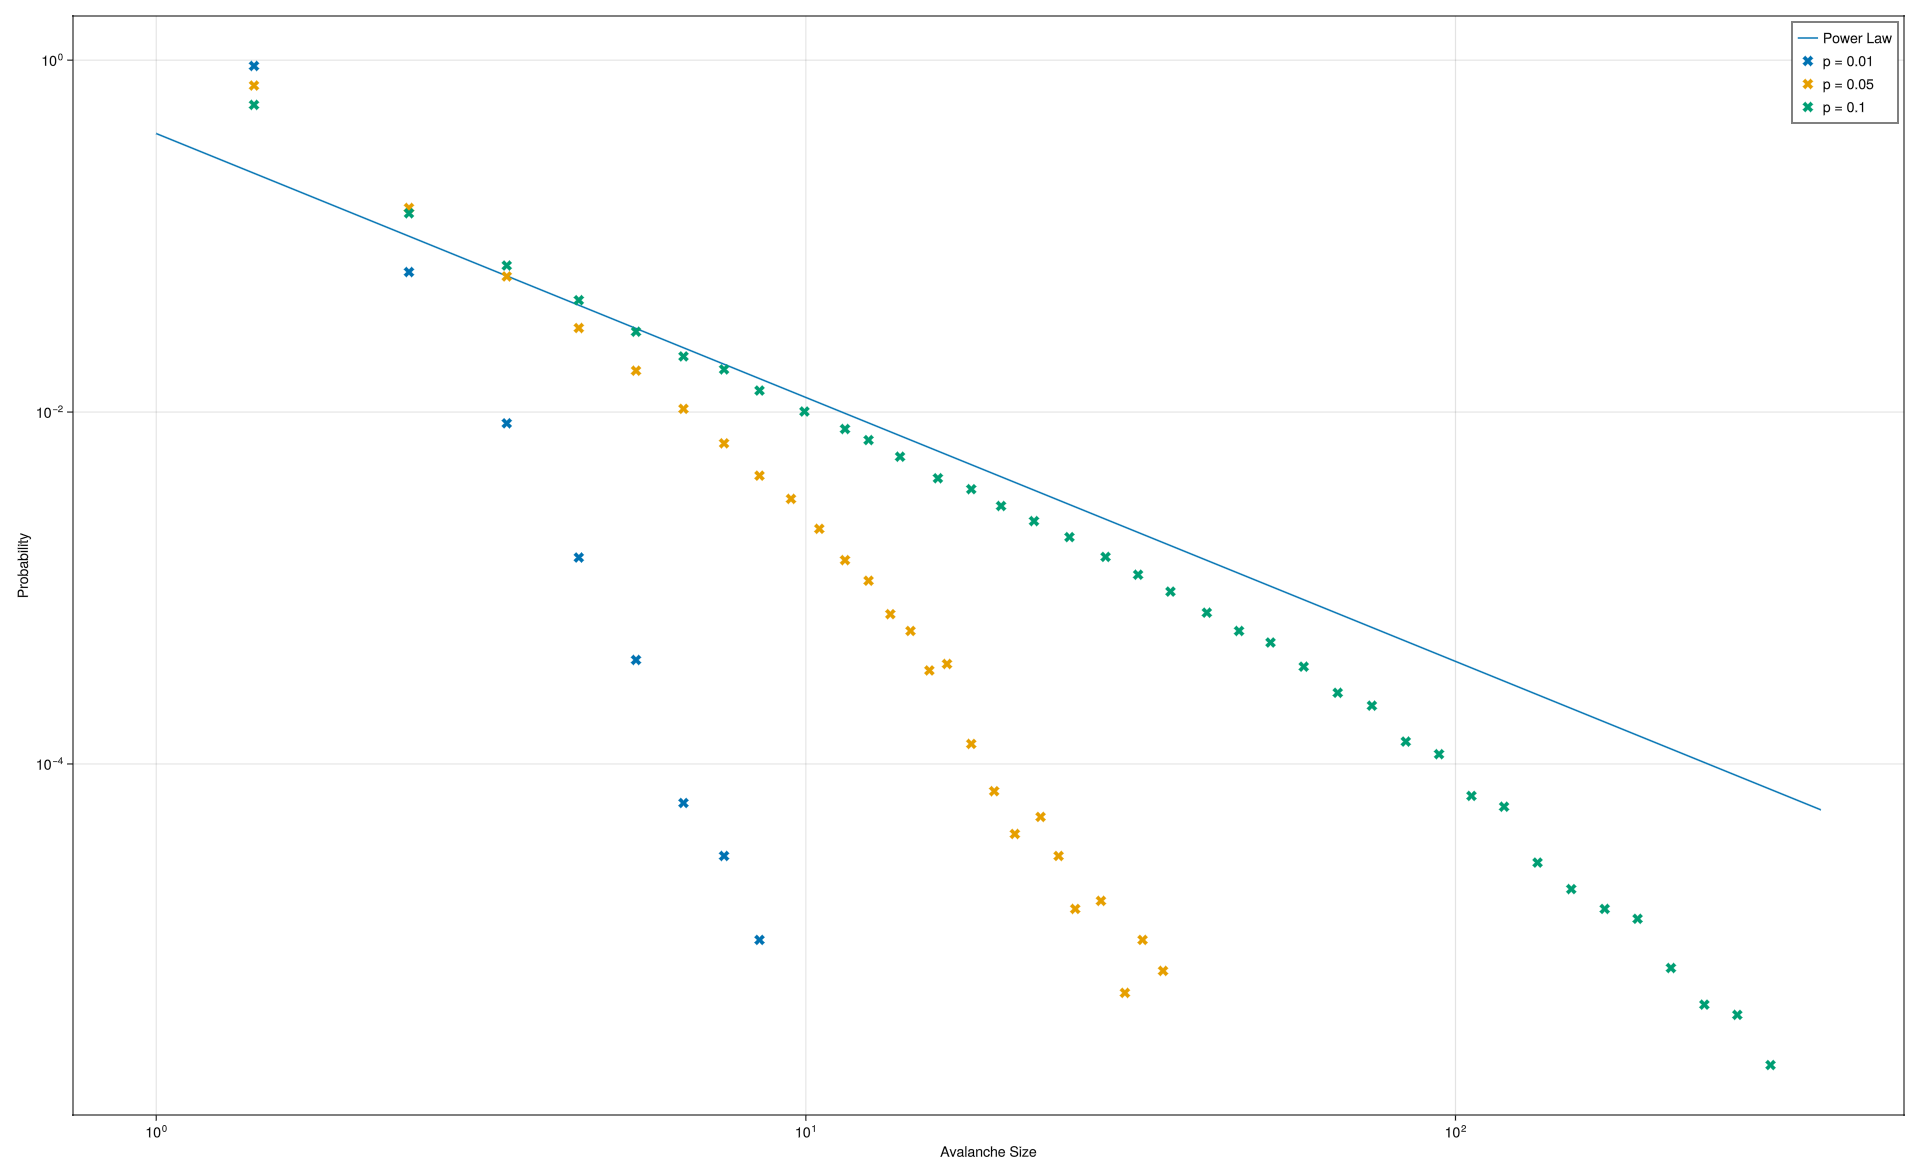
\includegraphics[width=.9\linewidth]{fig2.png}
\end{center}
Erdos-Reyni Network with Variable \(p\)
\begin{center}
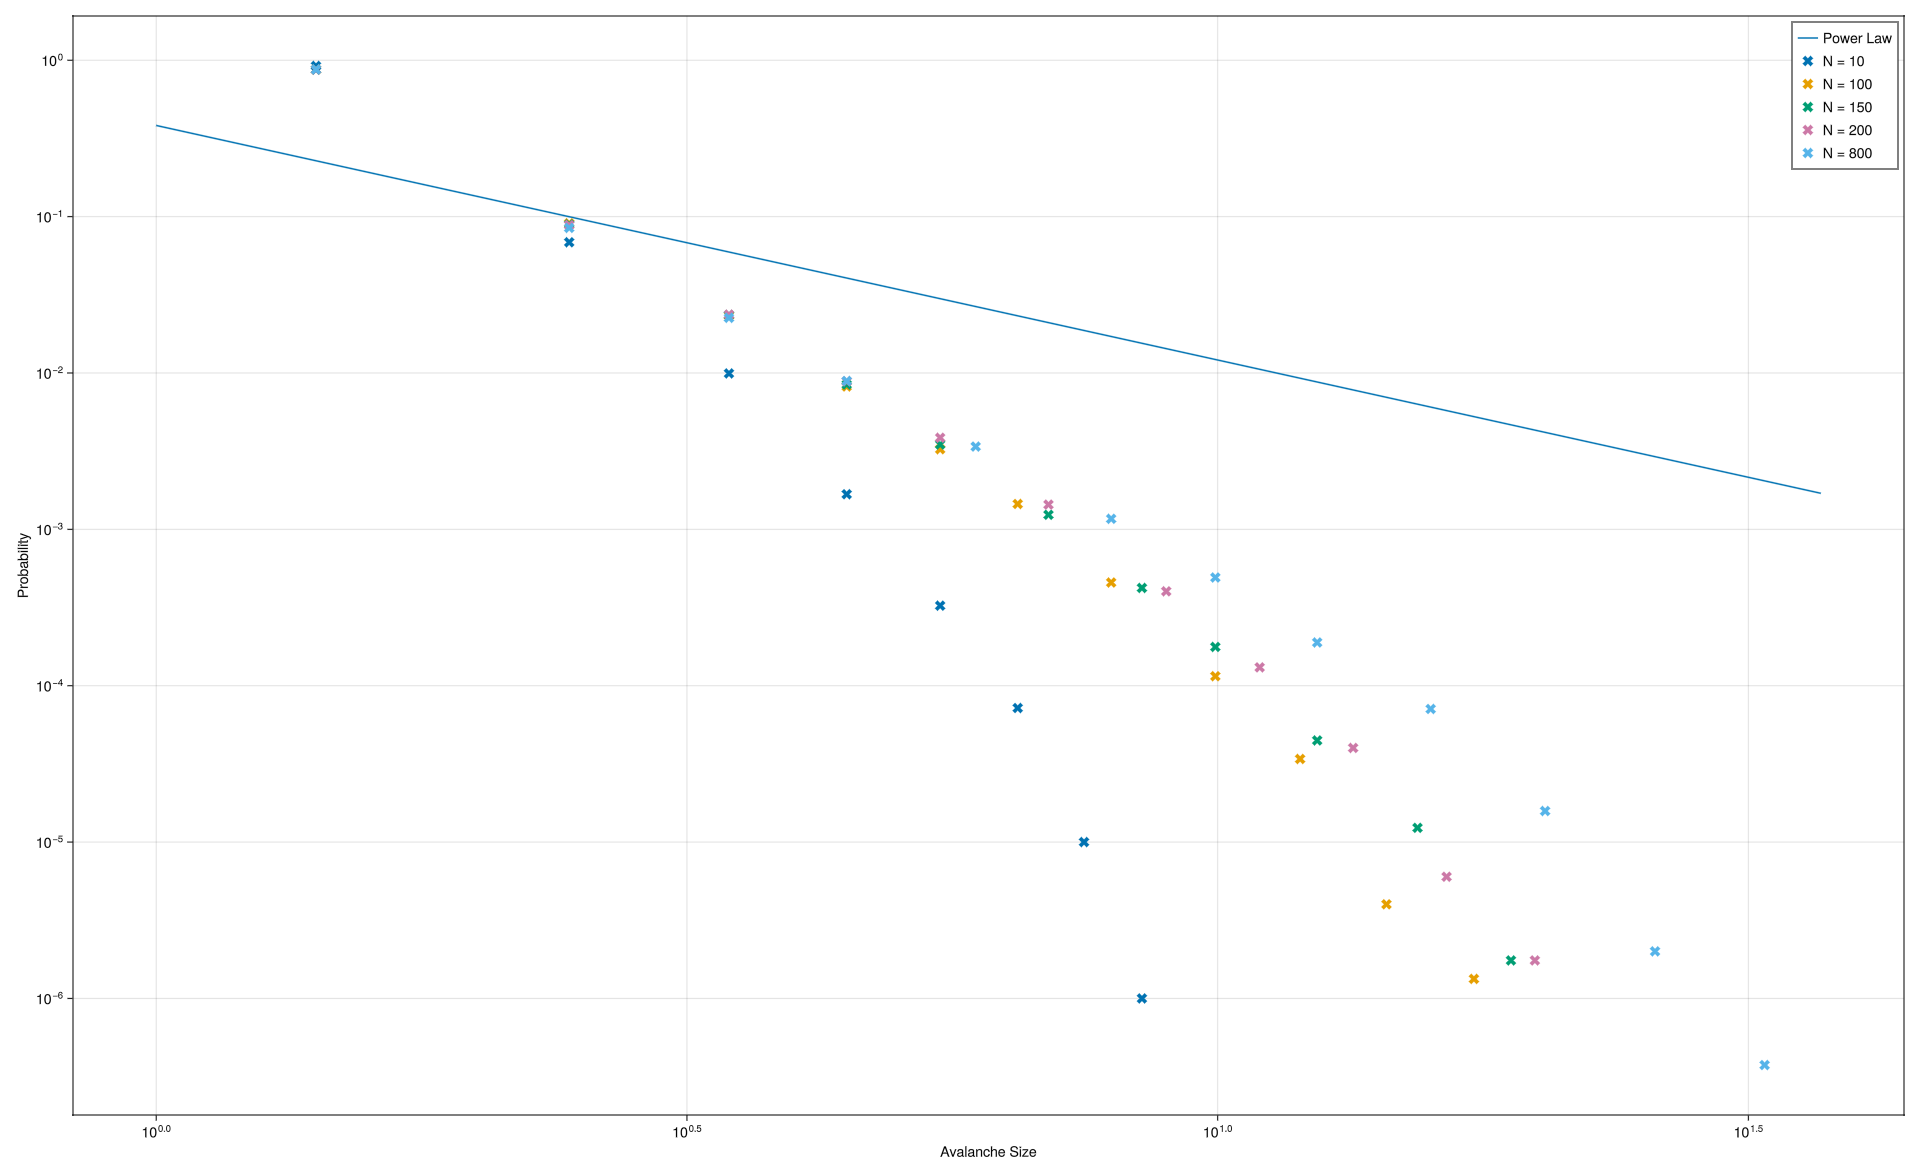
\includegraphics[width=.9\linewidth]{fig3.png}
\end{center}
Barabasi-Albert Network with Variable Size and \(m0=8\)
\end{center}

I'm still working on developing the software to quantitavely assess which probability distribution is appropriate. Once that's done I'll include those results as well.
\end{document}
